%----------------------------------------------------------------------------------------
%	PACKAGES AND OTHER DOCUMENT CONFIGURATIONS
%----------------------------------------------------------------------------------------
\documentclass[twoside]{article}

\usepackage[sc]{mathpazo} % Use the Palatino font
\usepackage[english]{babel}
\usepackage[utf8]{inputenc}
\usepackage{lipsum}
\usepackage{graphicx}
%\usepackage[T1]{fontenc} % Use 8-bit encoding that has 256 glyphs
\linespread{1.15} % Line spacing - Palatino needs more space between lines
\usepackage{microtype} % Slightly tweak font spacing for aesthetics

\usepackage[hmarginratio=1:1,top=32mm,columnsep=20pt]{geometry} % Document margins
\usepackage{multicol} % Used for the two-column layout of the document
\usepackage[hang, small,labelfont=bf,up,textfont=it,up]{caption} % Custom captions under/above floats in tables or figures
\usepackage{mathtools}
\usepackage{booktabs} % Horizontal rules in tables
\usepackage{float} % Required for tables and figures in the multi-column environment - they need to be placed in specific locations with the [H] (e.g. \begin{table}[H])
\usepackage{hyperref} % For hyperlinks in the PDF
\usepackage{wrapfig}
%\usepackage[]{mcode} % For embebing matlab code
\usepackage[makeroom]{cancel}

%\usepackage{lettrine} % The lettrine is the first enlarged letter at the beginning of the text
\usepackage{paralist} % Used for the compactitem environment which makes bullet points with less space between them

\usepackage{datetime}
\newdateformat{monthyeardate}{\monthname[\THEMONTH], \THEYEAR}
%\newdateformat{today}{\monthname[\THEMONTH], \date \THEYEAR}

\usepackage{abstract} % Allows abstract customization
\renewcommand{\abstractnamefont}{\normalfont\bfseries} % Set the "Abstract" text to bold
\renewcommand{\abstracttextfont}{\normalfont\small\itshape} % Set the abstract itself to small italic text

\usepackage{titlesec} % Allows customization of titles
%\renewcommand\thesection{\textbf{section}} % Roman numerals for the sections
%\renewcommand\thesubsection{\Roman{subsection}} % Roman numerals for subsections
\titleformat{\section}[block]{\large\scshape\centering}{\thesection.}{1em}{} % Change the look of the section titles
\titleformat{\subsection}[block]{\large\centering}{\thesubsection.}{1em}{} % Change the look of the section titles

\usepackage{fancyhdr} % Headers and footers
\pagestyle{fancy} % All pages have headers and footers
\fancyhead{} % Blank out the default header
\fancyfoot{} % Blank out the default footer
\fancyhead[C]{Astronomy % based on TRACS 
\hspace{4pt} $\bullet$ \hspace{4pt} The Period of the Sun
\hspace{4pt} $\bullet$ \hspace{4pt} \monthyeardate\today} % Custom header text
\fancyfoot[RO,LE]{\thepage} % Custom footer text

\usepackage{cite}

\DeclareGraphicsExtensions{.pdf,.png,.jpg} % Graphics type

%----------------------------------------------------------------------------------------
%	   TITLE SECTION
%----------------------------------------------------------------------------------------

\title{
	\vspace{-15mm}
	\fontsize{28pt}{10pt}
	\selectfont\textbf{The Period of Rotation of the Sun}% Article title
}

\author{
	\large
	\textsc{Jaime Díez González-Pardo}\\[4mm]%\thanks{A thank you or further information}\\[2mm] % Your name
	\fontsize{28pt}{10pt} University of Cantabria \\ % Your institution
	%\thanks{A thank you or further information}\\[2mm] % Your name
	\normalsize Astronomy \\ 
	%\normalsize{Compañera:} \textsc{Mónica Escobedo}\\%\normalsize \href{mailto:john@smith.com}{john@smith.com} % Your email address
	%\vspace{5mm}
}

\date{ \usdate\today }


%----------------------------------------------------------------------------------------
%      · DOCUMENT
%----------------------------------------------------------------------------------------

\begin{document}


	\maketitle % Insert title


	\thispagestyle{fancy} % All pages have headers and footers

%----------------------------------------------------------------------------------------
%	  ABSTRACT
%----------------------------------------------------------------------------------------

	\begin{abstract}

		\noindent% Dummy abstract text

		The rotation of the Sun has been studied by means of the apparent movement of 5 different sunspots over 11 days. Five different values for the Synodic and the Sideral period of rotation of the Sun have been calculated from longitudinal positions of sunspots obtaining the final value for each from their means. The synodic period obtained by susnpots near the equator is $(27.3 \pm 0.3) \textrm{ days}$ while the obtained for sunspot at latitude $>20$ degrees is $(28.46 \pm 0.04)$ days. The sideral period obtained by susnpots near the equator is $(25.4 \pm 0.2) \textrm{ days}$.

	\end{abstract}

%----------------------------------------------------------------------------------------
%	  ARTICLE CONTENTS
%----------------------------------------------------------------------------------------

	\begin{multicols}{2} % Two-column layout throughout the main article text

		\section{Introduction} % Scope of the project = rad effects + minimization

			Sunspots have been observed since many years before Galileo Galilei but he was the first to recorded the sunspots and observe how they move as the Sun rotated. This was a clear evidence that the Sun rotated, seen not only how these spots move, but they appear and disappear due to the spherical form of the Sun.

			The period of rotation of the Sun can be measured by means of the move of these sunspot studing how its positions changes over the time. Nevertheless, a discrepancy between the periods measured from spots near the equator and  the periods measured from spots further away the equator has been observed and explained as a consequence that the Sun is not a Solid body.

			However, this period of rotation of the Sun, called \textit{Synodic Period}, measured from the earth it is not exactly the period of rotation of the Sun due to the own rotation of the earth and due to its oibit around the Sun. For that reason the \textit{sidereal Period} is defined as the "true" rotation period of the Sun, which it is take respect to the distant stars.

		\section{Methods}

			In this experiment the CLEA program \textit{The Period of Rotation of the Sun} has been used to record the position of sunspots from 11 pictures of the Sun taken by the GONG solar telescopes.

				\begin{figure}[H]
					\centering
					\includegraphics[scale=0.135]{Figure/3.PNG}
					\caption{\label{Img:CLEA}The CLEA program \textit{The Period of Rotation of the Sun} used in the experiment with a picture of the Sun.}
				\end{figure}

			This program allows to obtain, save and plot the position of a certain point by means of its longitude and latitude coordinates. The positions on Heliographic Coordinates are given by the longitude and the latitude, measered in degrees. The latitude corresponds to the "height" over the Equator, been $0^o$ for the equator, positive above it and negative under it; of the Sun and the longitude runs right down the middle of the solar disk and take positive values to the rigth and negative to the left.

			Once the program has been started, the 11 pictures of the Sun of the GONG solar telescopes have been opened. The program provides these pictures by its own and characterize each one by their date and time of acquisition.

			When the first picture is opened, the longitude and latitude of each sunspot can be measured just by select the sunspot, as it is shown in Figure \ref{Img:CLEA}. The program also allowed to identify each sunspot by an ID so all the measurements are recorded with its ID, its Julian dates and its longitude and latitude.

			In this experiment five different sunspots have been measured, 4 of them near the equator and 1 at latitude $>20$ degrees, for each picture, repeating all the measurements each time.

			All the calculus have been done by a code script \cite{github}

		\section{Results}

			In Figure \ref{Img:sunspot} shows the 5 differents sunspot measured with its correspondent label. All the pictures used were taken between January $13^{th}$ and January $23^{rd}$ of 2002.	

				\begin{figure}[H]
					\centering
					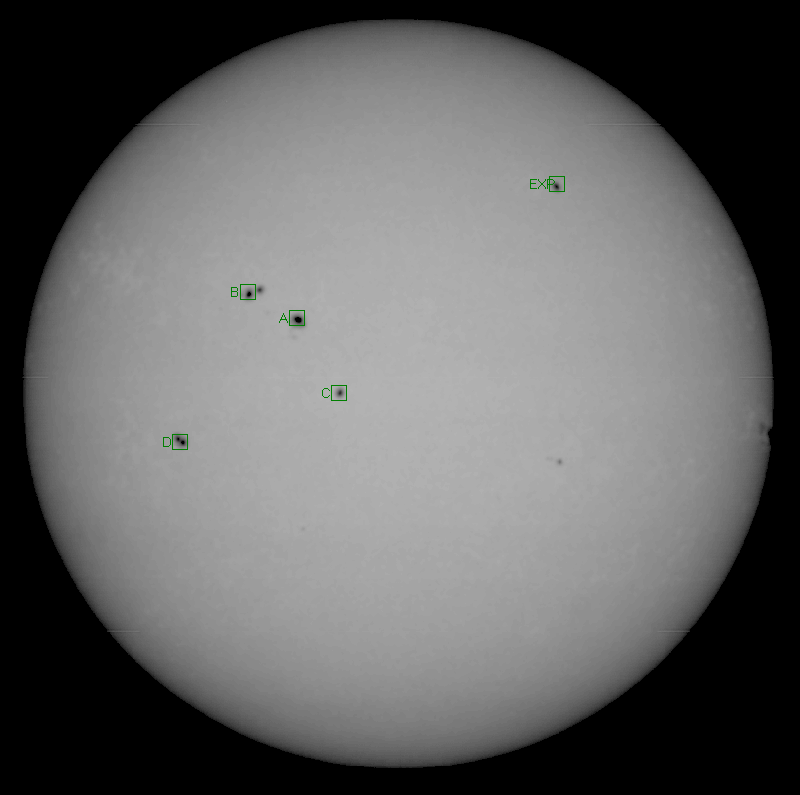
\includegraphics[scale=0.3]{Figure/sunspots.PNG}
					\caption{\label{Img:sunspot}Image of the Sun with the 5 sunspot used to obtain the synodic period of the Sun. Sunspots $A,B,C \textrm{ and }D$ are approximately at latitudes $<10$ degrees while sunspot $Esp$ is at latitude $>20$ degrees.}
				\end{figure}

			Measurements have been taken from 11 differents pictures of the Sun in differents days. However, sunspot $C$ disappear in the last one so it was only possible to take 10 measurements. Similarly, only 7 measurements have been taken for sunspot $Esp$. All the measurements taken are shown in the appendix \ref{sec:data}. 

			In Figure \ref{Img:Slopes} latitudes are plotted versus time of each sunspot.

				\begin{figure}[H]
					\centering
					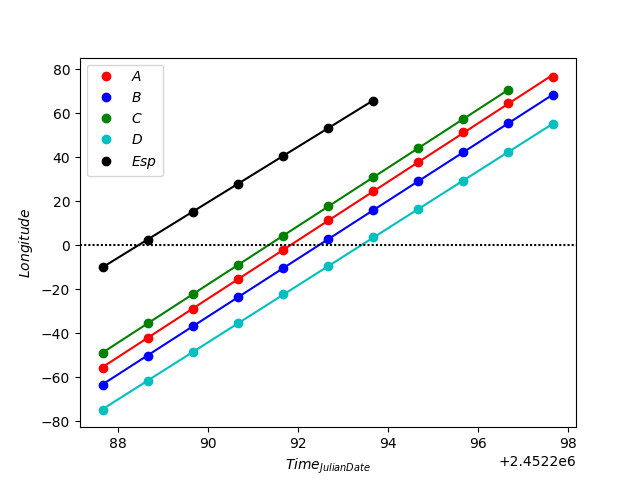
\includegraphics[scale=0.5]{Figure/Figure.png}
					\caption{\label{Img:Slopes}Latitudes versus time for each sunspot. The black one corresponds to sunspot at latitude $>20$ degrees. Values have been adjust by linear regression, slopes are shown in Table \ref{Tab:Slopes}.}
				\end{figure}

			Slopes shown in Table \ref{Tab:Slopes} represent how many degrees the Sun rotates per day.

				


			Synodic period of rotation of the Sun can be obtained by divide the $360^o$ degrees of the sphere over slopes $Synodic_{period} = \frac{360}{Slope}$. Synodic periods of each sunspot are shown in Table \ref{Tab:Synodic}.

				\begin{table}[H]
	\centering
	\begin{tabular}{ c c c}
		\hline
		\centering
			$Sunspot$ & $P_{Synodic}/days$ & $\sigma_{P_{sync}}/days$ \\\hline
			A & 27.04 & 0.08 \\
			B & 27.28 & 0.02 \\
			C & 27.10 & 0.03 \\
			D & 27.69 & 0.05 \\
			Esp & 28.46 & 0.04 \\\hline
	\end{tabular}
	\caption{\label{Tab:Synodic}Synodic period of rotation of the Sun, $P_{Synodic}$ for each sunspot with its standard deviation $\sigma_{P_{sync}}$.}
\end{table}


			In order to obtain an unique value for the synodic period the mean of all the obtained values has been calculated with its standard deviation.

				\begin{equation}
					\bar{P}_{synodic} = \sum_N P_{synodic_N} = (27.5 \pm 0.5) \textrm{ days}
					\label{eq:SynodicMean}
				\end{equation}

			However, due to discrepancy between values obtained for sunspot at latitudes $<10$ and the value obtained from the $Esp$ sunspot at latitude $>20$ degrees, $\bar{P}_{synodic}$ is calculated again but without $Esp$'s value.

				\begin{equation}
					\bar{P}_{synodic} = \sum_{N-1} P_{synodic_N} = (27.3 \pm 0.3) \textrm{ days}
					\label{eq:SynodicMeanWhitout}
				\end{equation}

			Sidereal period of rotation od the Sun can be calculated from synodic period with following equation.

				\begin{equation}
					P_{sidereal}=  (P_{synodic} \cdot 365.25) / (P_{synodic} + 365.25) 
					\label{eq:Sideral}
				\end{equation}

			In order to obtain an unique value for the sidereal period of rotation of the Sun, the former method used for synodic period has been followed, obtaining first the sideral period for each sunspot, and then, the mean value with and without $Esp$'s value.

			In Table \ref{Tab:Sideral} appear all sidereal periods obtained from synodic periods of Table \ref{Tab:Synodic} by equation \ref{eq:Sideral}.

				\begin{table}[H]
	\centering
	\begin{tabular}{ c c}
		\hline
		\centering
			$Sunspot$ & $P_{sideral}/days$ \\\hline
			A & 25.17 \\
			B & 25.38 \\
			C & 25.23 \\
			D & 25.74 \\
			Esp & 26.41 \\\hline
	\end{tabular}
	\caption{\label{Tab:Sideral}Sideral period of rotation of the Sun, $P_{sideral}$ for each sunspot calculated by the equation \label{eq:Sideral}.}
\end{table}


				\begin{equation}
					\bar{P}_{sidereal} = \sum_N P_{sidereal_N} = (25.6 \pm 0.5) \textrm{ days}
						\label{eq:sideralMean}
				\end{equation}

				\begin{equation}
						\bar{P}_{sidereal} = \sum_{N-1} P_{sidereal_N} = (25.4 \pm 0.2) \textrm{ days}
						\label{eq:sideralMeanWhitout}
					\end{equation}

		\section{Conclussions}

			The position (latitude and longitude) of 5 sunspots have been measured from 11 pictures of the Sun took at different days, been able to observe how susnpots move over time due to the rotation of the Sun. 

			Latitude magnitud does not change a lot over the time but for sunspot $B$ some important fluctuations have been observe. These fluctuations along latitude could also affect the longitude measurements.

			The period of rotation of the Sun has been obtained from the longitude values obtaining first the synodic period for the 4 sunspot near the equator ($27.3 \pm 0.3 \textrm{ days}$) and for the sunspot at latitude $<20$ degrees ($28.46 \pm 0.04$ days). This discrepancy between the values is not possible if the Sun were a solid body and agree with the theory and it is called differential rotation. The sidereal period obtained for the near equator susnpots is $(25.6 \pm 0.5) \textrm{ days}$.

			The errors obtained from the standard deviation of the means are one order of magnitude bigger than obtained from the standard deviation of the linear deviation. This discrepancy shows that although the logitude of the sunspot evolves as a linear function, the slopes , and so the periods, obtained vary for each sunspots. However, this error is also very good been around $2\%$. When the values from the sunspot at latitude $<20$ degrees are not considered for the mean, the standard deviation also decrese.

	\end{multicols}

%----------------------------------------------------------------------------------------
%     BIBLIOGRAPHY
%----------------------------------------------------------------------------------------

	\bibliographystyle{unsrt}
	\bibliography{../../biblio}

%----------------------------------------------------------------------------------------
%     APPENDIX
%----------------------------------------------------------------------------------------
	\newpage
		\appendix

		\section{Tables with all measurements}
			\label{sec:data}

			\begin{multicols}{2}

				\begin{table}[H]
	\centering
	\begin{tabular}{ c  c  c }
		\\\hline
		\centering
			$Time_{Julian Date}$ & $Longitude_{A}$ & $Latitude_{A}$ \\\hline
			2452287.66685 & -55.65453 & 6.55383 \\
			2452288.66685 & -42.2863 & 6.5937 \\
			2452289.66685 & -28.8823 & 6.64063 \\
			2452290.66685 & -15.50355 & 6.67726 \\
			2452291.66685 & -2.01846 & 6.70327 \\
			2452292.66685 & 11.37515 & 6.62191 \\
			2452293.66685 & 24.77242 & 6.60149 \\
			2452294.66685 & 38.04959 & 6.41166 \\
			2452295.66685 & 51.31593 & 6.29824 \\
			2452296.66685 & 64.83209 & 6.62467 \\
			2452297.66685 & 76.66677 & 6.57176 \\\hline
	\end{tabular}
	\caption{\label{Tab:sunspotA}Longitude and latitude of sunspot $A$ in function of the time, in Julian date, at each picture of the Sun measured.}
\end{table}

				\begin{table}[H]
	\centering
	\begin{tabular}{ c  c  c }
		\\\hline
		\centering
			$Time_{Julian Date}$ & $Longitude_{B}$ & $Latitude_{B}$ \\\hline
			2452287.66685 & -63.34676 & 11.23107 \\
			2452288.66685 & -50.18665 & 11.08985 \\
			2452289.66685 & -36.88429 & 10.9511 \\
			2452290.66685 & -23.58993 & 10.87732 \\
			2452291.66685 & -10.41042 & 10.75143 \\
			2452292.66685 & 2.80314 & 10.59884 \\
			2452293.66685 & 16.0277 & 10.33038 \\
			2452294.66685 & 29.2019 & 10.09961 \\
			2452295.66685 & 42.40231 & 10.01009 \\
			2452296.66685 & 55.40194 & 10.0055 \\
			2452297.66685 & 68.5707 & 9.97334 \\\hline
	\end{tabular}
	\caption{\label{Tab:sunspotB}Longitude and latitude of sunspot $B$ in function of the time, in Julian date, at each picture of the Sun measured.}
\end{table}

			\end{multicols}
			
			\begin{multicols}{2}
				\begin{table}[H]
	\centering
	\begin{tabular}{ c  c  c }
		\\\hline
		\centering
			$Time_{Julian Date}$ & $Longitude_{C}$ & $Latitude_{C}$ \\\hline
			2452287.66685 & -48.83466 & -4.97057 \\
			2452288.66685 & -35.5057 & -4.77817 \\
			2452289.66685 & -22.32334 & -4.60597 \\
			2452290.66685 & -9.04038 & -4.51789 \\
			2452291.66685 & 4.19704 & -4.45484 \\
			2452292.66685 & 17.66659 & -4.46922 \\
			2452293.66685 & 31.04852 & -4.5463 \\
			2452294.66685 & 44.35606 & -4.5057 \\
			2452295.66685 & 57.51859 & -4.40233 \\
			2452296.66685 & 70.43497 & -4.44667 \\\hline
	\end{tabular}
	\caption{\label{Tab:sunspotC}Longitude and latitude of sunspot $C$ in function of the time, in Julian date, at each picture of the Sun measured.}
\end{table}

				\begin{table}[H]
	\centering
	\begin{tabular}{ c  c  c }
		\\\hline
		\centering
			$Time_{Julian Date}$ & $Longitude_{D}$ & $Latitude_{D}$ \\\hline
			2452287.66685 & -75.09 & -10.39144 \\
			2452288.66685 & -61.52851 & -10.6506 \\
			2452289.66685 & -48.42289 & -10.90289 \\
			2452290.66685 & -35.34592 & -11.11281 \\
			2452291.66685 & -22.33181 & -11.18763 \\
			2452292.66685 & -9.39826 & -11.38654 \\
			2452293.66685 & 3.61386 & -11.52341 \\
			2452294.66685 & 16.5406 & -11.55453 \\
			2452295.66685 & 29.43427 & -11.62974 \\
			2452296.66685 & 42.40014 & -11.70924 \\
			2452297.66685 & 55.16223 & -11.70424 \\\hline
	\end{tabular}
	\caption{\label{Tab:sunspotD}Longitude and latitude of sunspot $D$ in function of the time, in Julian date, at each picture of the Sun measured.}
\end{table}

			\end{multicols}

			\begin{table}[H]
	\centering
	\begin{tabular}{ c  c  c }
		\\\hline
		\centering
			$Time_{Julian Date}$ & $Longitude_{Esp}$ & $Latitude_{Esp}$ \\\hline
			2452287.66685 & -10.06711 & 28.79832 \\
			2452288.66685 & 2.59907 & 28.69309 \\
			2452289.66685 & 15.32213 & 28.81208 \\
			2452290.66685 & 27.96642 & 28.7478 \\
			2452291.66685 & 40.68168 & 28.52958 \\
			2452292.66685 & 53.31627 & 28.61809 \\
			2452293.66685 & 65.70861 & 28.58446 \\\hline
	\end{tabular}
	\caption{\label{Tab:sunspotEsp}Longitude and latitude of sunspot $Esp$ in function of the time, in Julian date, at each picture of the Sun measured.}
\end{table}



\end{document}

%--------------------------------------------------------------------------------------
%            TEMPLATES
%--------------------------------------------------------------------------------------

%----------------------------------------------------------------------------------------
%            how to insert an image
%----------------------------------------------------------------------------------------

%	\begin{figure}[H]
%		\centering
%		\includegraphics[scale= ]{nombre de la imagen.jpg}
%		\caption{\label{Img:widgets}el pie de pagina que le quieras 	poner a la imagen}
%	\end{figure}
 
%----------------------------------------------------------------------------------------
%            how to insert a table
%----------------------------------------------------------------------------------------

%	\begin{table}[H]
%		\centering
%		\begin{tabular}{|c|c|c|c|}
%			\hline
%			\centering
%				Altura(h) & Distancia (d) & Elaboracion (e) & Longitud (l) \\
%				($\pm0.5$ mm) & ($\pm0.5$ mm) & ($\pm0.5$ mm) & ($\pm0.5$ mm) \\ \hline
%				 &  &  &  \\ \hline
%				 &  &  &  \\ \hline
%				 &  &  &  \\ \hline
%				 &  &  &  \\ \hline
%				 &  &  &  \\ \hline
%		         &  &  &  \\ \hline
%		\end{tabular}
%		\caption{\label{Tab:widgets}pie de pagina que le quieras poner}
%	\end{table}

%----------------------------------------------------------------------------------------
%             How to remove the label in equactions
%----------------------------------------------------------------------------------------

%	\begin{equation*}
%		
%	\end{equation*}

%----------------------------------------------------------------------------------------
%              How to set bibliography
%----------------------------------------------------------------------------------------

%\bibliographystyle{unsrt}
%\bibliography{biblio}
%
%Then you have to set a .bib document such as the next template
%
%	@book{nickname,
%	author = {},
%	title = {},
%	edition = {},
%	year = {},
%	volume = {},
%	ISBN = {}
%	}
%
%	@ARTICLE{nickname,
%	author = {},
%	title = {},
%	year = {},
%	volume = {},
%	}


%----------------------------------------------------------------------------------------
%              END
%----------------------------------------------------------------------------------------